

\section{O pensamento musical na Antigüidade
clásica}\label{o-pensamento-musical--na-antiguxfcidade-cluxe1sica}

Como noutros ámbitos, tamén na música, as antigas civilizacións grega e
romana puxeron as bases da cultura europea posterior. Pero esta
influencia non se deu tanto na música práctica como no pensamento
musical: as ideas e teorías desenvolvidas na antiga Grecia mantivéronse
vivas ata o Renacemento; e non só no pensamento musical da Europa
latina, senón tamén nas culturas bizantina e árabe.

A palabra grega \emph{musiké} significaba «relativo ás musas».
As musas, nos relatos míticos, eran nove e estaban relacionadas con
actividades como a poesía, a historia, a traxedia, a comedia ou a danza.
Todas estas actividades englobábanse baixo o concepto de \emph{musiké} ,
que comprendía por tanto a música, a poesía (lírica, épica e dramática)
e a danza. A música, pois, era para os antigos gregos unha actividade
moito máis diversa que o que o termo designa na nosa cultura.


\subsection*{Concepto matemático da
música}\label{concepto-matemuxe1tico-da-muxfasica}

A base do pensamento musical grego atopámola na escola pitagórica,
formada polos discípulos de Pitágoras \textbf{de Samos}, que viviu no
século VI a.C., e é por tanto un dos filósofos chamados
\emph{presocráticos}. Os pitagóricos, que non só compartían unha serie
de ideas filosóficas, senón tamén un estilo de vida común, defendían que
o universo enteiro ten unha estrutura matemática, que todo se reduce a
número. Aínda que Pitágoras non deixou nada escrito, os seus discípulos
transmitiron as súas teorías; sabemos así que Pitágoras realizou unha
serie de experimentos con obxectos sonoros, descubrindo que o tres
intervalos básicos da música grega (oitava, quinta e cuarta)
correspondían a tres proporciones simples:

\begin{center}
\begin{tabular}{lll}
Intervalo & Nome grego & Proporción \\
Oitava & \emph{Diapasón} & 2:1 \\
Quinta & \emph{Diapente} & 3:2 \\
Cuarta & \emph{Diatessaron} & 4:3 \\
\end{tabular}
\end{center}

É dicir, se unha corda tocada ao aire produce unha nota determinada, ao
pulsar no seu centro e facer vibrar a metade da corda soaría a súa
oitava; se facemos vibrar os dous terzos, soaría a súa quinta; e se
facemos vibrar o tres cuartos, soaría a súa cuarta. O mesmo pódese
aplicar ás lonxitudes dos tubos sonoros e a moitos outros obxectos que
producen notas.

\begin{figure}
\centering
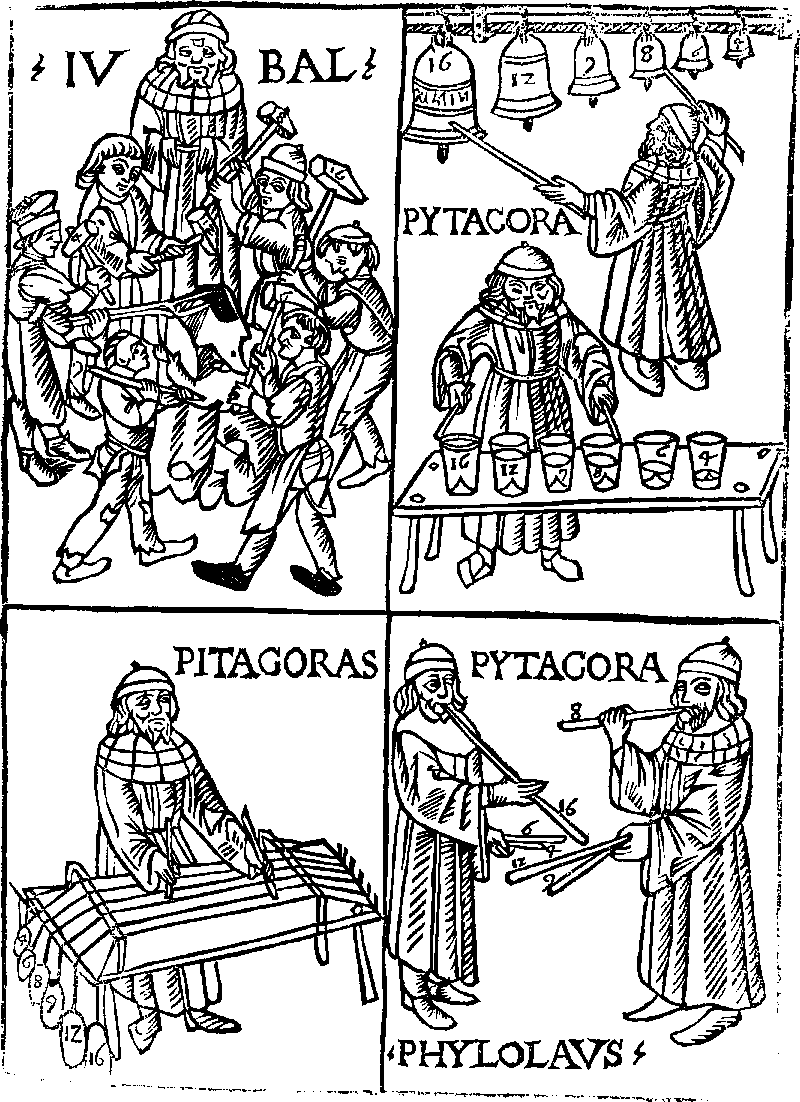
\includegraphics[width=0.70\textwidth]{/ud-01/pitagoras.png}
\caption{Gravado publicado en Theorica  musicae, de Franchino Gaffurio, en 1492}
\end{figure}

Por tanto, os intervalos básicos da música grega (e despois a occidental
e moitas outras) corresponden ás proporcións da serie 1:2:3:4, formada
polo catro primeiros números naturais, cuxa suma é dez, e que para os
pitagóricos representaba a perfección, simbolizada gráficamente na
\emph{tetraktys}:

\begin{wrapfigure}{l}{0.30\textwidth}
\begin{center}
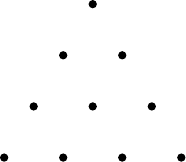
\includegraphics[width=0.20\textwidth]{/ud-01/tetraktys.png}
\end{center}
\caption{\emph{Tetraktys}}
\end{wrapfigure}

Á marxe do significado místico ou esotérico que estas proporcións
tivesen para os pitagóricos, o seu descubrimento tivo unha importante
aplicación práctica na afinación vocal e instrumental durante a este
período e a Idade Media: todos os demais intervalos calculábanse a
partir das tres proporciones indicadas. Ademais, o estudo da música
considerouse parte das matemáticas, incluíndose ao final da Idade Antiga
no que se denominou \emph{Quadrivium}: Aritmética, Xeometría, Astronomía
e Música, o conxunto do catro disciplinas matemáticas que conformaban a
educación superior (e que se mantería durante a Idade Media).

\begin{figure}
\centering
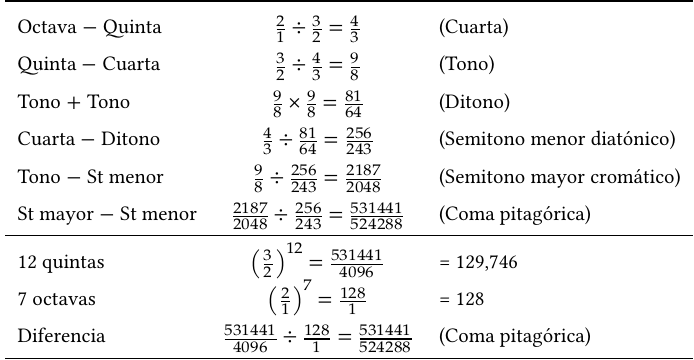
\includegraphics{/ud-01/proporciones.png}
\caption{Cálculo de intervalos a partir das proporcións pitagóricas.}
\end{figure}

A diferenza entre as doce quintas e as sete oitavas mostra a
inexistencia dun verdadeiro «círculo de quintas».


\subsection*{A harmonía das esferas}\label{a-harmonuxeda-das-esferas}

A imaxe cosmolóxica da antigüidade expuña un universo coa Terra no seu
centro, rodeada de sucesivas esferas concéntricas nas que se inserían os
«planetas», os astros coñecidos entón: a Luna, Mercurio, Venus, o Sol,
Marte, Júpiter e Saturno. Unha oitava esfera contiña as estrelas. Todas
estas esferas viraban ao redor da Terra a velocidades diferentes. Os
gregos sabían que o son procede do movemento, polo que pensaban que o
movemento de cada esfera debía producir un son distinto; dado que,
segundo as teorías pitagóricas, as distancias entre as esferas
coincidían coas proporcións simples da música, o conxunto dos sons do
oito esferas configuraba unha \emph{harmonía}, unha melodía que soa
constantemente: a \emph{harmonía das esferas.} Algúns chegaron mesmo a
expor que notas correspondían a cada esfera, aínda que nisto nunca houbo
un modelo predominante.

\begin{figure}[htp]
\centering
\includegraphics[width=0.50\textwidth]{/ud-01/esferas2.png}
\caption{O modelo cosmolóxico xeocéntrico, tal como se concibía na Idade Media}
\end{figure}

%\begin{wrapfigure}{l}{0.30\textwidth}
%\begin{center}
%\includegraphics[width=0.60\textwidth]{/home/robertoprado/Documentos/GitHub/Historia-I/figures/ud-01/esferas2.png}
%\end{center}
%\caption{O modelo cosmolóxico xeocéntrico, tal como se concibía na Idade Media}
%\end{wrapfigure}

Posto que a música é un reflexo da estrutura do cosmos, o estudo das
proporcións matemáticas dos intervalos era un medio para pescudar esa
estrutura. Isto levou a un estudo exhaustivo destas proporcións que se
mantivo durante toda a historia da música grega e pasou á Idade Media a
través da obra de Boecio. Os teóricos musicais medievais e renacentistas
seguiron desenvolvendo modelos matemáticos dos intervalos que estiveron
moi presentes nos nuevo sistemas de afinación que conduciron á escala
temperada. Mesmo no século XVII, cando Johannes Kepler enunciou as leis
do movemento dos planetas, seguía afirmando que estes producían sons ao
moverse.

A visión matemática da música segue sendo tema de estudo na actualidade,
con aplicacións como \emph{a música fractal}.


\subsection*{\texorpdfstring{Teoría do
\emph{ethos}}{Teoría do ethos}}\label{teoruxeda-do--ethos}

Do mesmo xeito que o cosmos, o ser humano tamén está composto de
proporcións matemáticas, que regulan a relación entre corpo e alma e
entre cada parte desta. Por tanto, a música pode reflectir a estrutura
psíquica dun ser humano, e así se relaciona cos diferentes estados de
ánimo.

A partir desta concepción expúxose que a música podía modelar o
comportamento dunha persoa se se utilizaba conscientemente no seu
proceso de formación; diferentes músicas podían configurar diferentes
personalidades. Damón, no século V a.C., clasificou as \emph{harmoníai}
da súa época segundo os seus efectos na personalidade, relacionando
deste xeito cada música cun comportamento ou \emph{ethos}
determinado. As teorías de Damón foron recollidas por Platón.

A teoría do \emph{ethos} causou unha intensa polémica entre os seus
defensores e os seus detractores, o cal levou na época helenística a
unha diverxencia cada vez maior entre músicos e teóricos ---que
continuaría na Idade Media--- e ao abandono progresivo da propia teoría.
Con todo, as épocas de neoplatonismo rescatárona, principalmente a
finais da Idade Antiga e sobre todo no Renacemento, cando foi o xerme da
\emph{teoría dos afectos} que dominou a estética barroca.

Na actualidade hai visións da música próximas á teoría do \emph{ethos},
como pode ser a musicoterapia.

